\documentclass[final,1p,times,number,amsthm]{elsart}
\journal{Journal of Symbolic Computation}



\usepackage[utf8x]{inputenc}
\usepackage{yjsco}
\usepackage{natbib}
\usepackage{amsmath}
\usepackage{amsfonts}
\usepackage{amssymb}
\usepackage{amsthm}
\usepackage{fontenc}
\usepackage{graphicx}
\usepackage{bbm}
\usepackage{tikz}
\usepackage{todonotes}
\usepackage{multirow}
\usepackage[colorlinks]{hyperref}



\newtheorem{lemma}{Lemma}
\newtheorem{theorem}[lemma]{Theorem}
\newtheorem{corollary}[lemma]{Corollary}
\newtheorem{example}[lemma]{Example}
\newtheorem{definition}[lemma]{Definition}
\newtheorem{proposition}[lemma]{Proposition}
\newtheorem{remark}[lemma]{Remark}

\usetikzlibrary{patterns,decorations.pathreplacing}

\newlength\thickness
\pgfdeclarepatternformonly[\thickness]{section}
{\pgfpointorigin}{\pgfpoint{0.2cm}{0.2cm}}{\pgfpoint{0.2cm}{0.2cm}}
{
  \pgfsetlinewidth{\thickness}
  \pgfpathmoveto{\pgfpoint{0cm}{0cm}}
  \pgfpathlineto{\pgfpoint{1cm}{1cm}}
  \pgfpathclose
  \pgfsetlinewidth{\thickness}
  \pgfpathmoveto{\pgfpoint{0cm}{.5cm}}
  \pgfpathlineto{\pgfpoint{.5cm}{1cm}}
  \pgfpathclose
  \pgfsetlinewidth{\thickness}
  \pgfpathmoveto{\pgfpoint{.5cm}{0cm}}
  \pgfpathlineto{\pgfpoint{1cm}{.5cm}}
  \pgfusepath{stroke}
}

\pgfdeclarepatternformonly[\thickness]{section2}
{\pgfpointorigin}{\pgfpoint{1cm}{1cm}}{\pgfpoint{1cm}{0.2cm}}
{
  \pgfsetlinewidth{\thickness}
  \pgfpathmoveto{\pgfpoint{0cm}{1cm}}
  \pgfpathlineto{\pgfpoint{1.0cm}{0.cm}}
  \pgfpathclose
  \pgfsetlinewidth{\thickness}
  \pgfpathmoveto{\pgfpoint{0cm}{.5cm}}
  \pgfpathlineto{\pgfpoint{.5cm}{1cm}}
  \pgfpathclose
  \pgfsetlinewidth{\thickness}
  \pgfpathmoveto{\pgfpoint{.5cm}{0cm}}
  \pgfpathlineto{\pgfpoint{1cm}{.5cm}}
  \pgfusepath{stroke}
}

\pgfdeclarepatternformonly[\thickness]{section3}
{\pgfpointorigin}{\pgfpoint{0.3cm}{0.3cm}}{\pgfpoint{0.15cm}{0.15cm}}
{
  \pgfsetlinewidth{0.3pt}
  \pgfpathmoveto{\pgfqpoint{0pt}{0pt}}
  \pgfpathlineto{\pgfqpoint{3pt}{3pt}}
  \pgfpathmoveto{\pgfqpoint{0pt}{3pt}}
  \pgfpathlineto{\pgfqpoint{3pt}{0pt}}
  \pgfusepath{stroke}
}

\pgfdeclarepatternformonly[\thickness]{section4}{\pgfqpoint{-1pt}{-1pt}}
{\pgfqpoint{4pt}{4pt}}{\pgfqpoint{\thickness}{\thickness}}
{
  \pgfsetlinewidth{0.3pt}
  \pgfpathmoveto{\pgfqpoint{0pt}{0pt}}
  \pgfpathlineto{\pgfqpoint{0pt}{3.1pt}}
  \pgfpathmoveto{\pgfqpoint{0pt}{0pt}}
  \pgfpathlineto{\pgfqpoint{3.1pt}{0pt}}
  \pgfusepath{stroke}
}

\tikzset{
  thickness/.store in = \thickness,
  thickness = 0.5pt
}




\let\set\mathbbm
\newcommand{\cfield}{\mathbbm{C}}
\newcommand{\nv}{n}
\newcommand{\ns}{\ell}
\newcommand{\ps}[2]{\cfield[[x_{#1},\dots,x_{#2}]]}
\newcommand{\psloc}[2]{\cfield((x_#1,\dots,x_#2))}
\newcommand{\psfield}[2]{\operatorname{Frac}(\cfield((x_#1,\dots,x_#2)))}
\newcommand{\pder}[2]{\frac{\partial}{\partial #2}#1}
\newcommand{\xqedhere}[2]{\rlap{\hbox to#1{\hfil\llap{\ensuremath{#2}}}}}




\begin{document}

\begin{frontmatter}

\date{\today} \title{Formal Solutions of Completely Integrable Pfaffian Systems
  With Normal Crossings}

\author{Barkatou, Moulay A.}
\address{XLIM UMR 7252 , DMI, University of Limoges; CNRS\\
        123, Avenue Albert Thomas, 87060 Limoges, France\\
        \texttt{moulay.barkatou@unilim.fr}}

 \author{Jaroschek, Maximilian}
 \address{Max Planck Institute for Informatics,\\ Saarbruecken, Germany\\
  \texttt{maximilian@mjaroschek.com}}

\author{Maddah, Suzy S.}
\address{Fields Institute\\
  222 College St, Toronto, ON M5T 3J1 Ontario, Canada\\
  \texttt{suzy.maddah@inria.fr}}


\begin{abstract}
  In this paper, we present an algorithm for computing a fundamental matrix of
  formal solutions of completely integrable Pfaffian systems with normal
  crossings in several variables. This algorithm is a generalization of a method
  developed for the bivariate case based on a combination of several reduction
  techniques and is partially\footnote{Our Maple package PfaffInt can be
    downloaded at: \url{http://www.mjaroschek.com/pfaffian/} It contains
    functionalities illustrated by examples for the splitting, column reduction,
    rank reduction, and the computation of exponential parts of multivariate
    completely integrable systems with normal crossings}implemented in the
  computer algebra system \textsc{Maple}.
\end{abstract}

\begin{keyword}
  Linear systems of partial differential equations, Pfaffian systems, Formal
  solutions, Rank reduction, Hukuhara-Turrittin's normal form, Normal crossings.
\end{keyword}

\end{frontmatter}



\section{Introduction}
\label{sec:intro}
Pfaffian systems arise in many applications~\cite{key74}, including the studies
of aerospace, celestial mechanics~\cite{key31}, and
statistics~\cite{key3062}. So far, the most important systems for applications
are those with so-called normal crossings~\cite{key32}.

A univariate completely integrable Pfaffian system with normal crossings reduces
to a singular linear system of ordinary differential equations (ODS, in short),
which have been studied extensively (see~\cite{key6,key7} and references
therein). Moreover, unlike the general case of several variables considered
herein, algorithms to related problems leading to the computation of formal
solutions have been developed by various authors
(see~\cite{key24,key40,key25,key26} and references therein). The \textsc{Maple}
package \textsc{Isolde}~\cite{key27} and \textsc{Mathemagix} package
\textsc{Lindalg}~\cite{key427} are dedicated to the symbolic resolution of such
systems.

More recently, bivariate systems were treated by the first and third author of
this paper in~\cite{key101}. This paper refines the results of the bivariate
case and generalizes them to treat the more general multivariate case.

To get an intuition of the kind of systems we consider, we informally study the
following simple bivariate completely integrable Pfaffian system with normal
crossings. A formal definition of these systems will be given in
Section~\ref{sec:prelim}.

\begin{example}~\cite[Example 2]{key101}
  \label{ex:sim}
  Given the following bivariate system over the ring of formal power series in
   with complex coefficients:
  
  we are interested in constructing the formal objects  that satisfy the
  system. The existence of a fundamental matrix of solutions and its general
  form follows from well known theoretical results (see
  Corollary~\ref{gerardsol}). The proof, however, is not constructive. For
  simplicity, we assume we already know that a fundamental matrix of formal
  solutions in our particular case is of the form
   where
   is a matrix with formal power series entries,  and 
  are matrices with entries in , and ,~ are polynomials in
   respectively. We now want to determine
  .  For this purpose, we use the algorithm
  presented in~\cite{key101}. The main idea is to compute one part
  of the solution by considering an associated ODS in only one variable and then
  use this information to compute the other parts of the solution by
  transforming and decoupling the system into smaller and simpler systems:

  \begin{itemize}
  \item First, we construct two associated systems whose equations are derived
    by setting either  or :
    
    We show in Section~\ref{sec:invariants} that the formal invariants  and  can be computed from these associated systems. Via
    \textsc{Isolde} or \textsc{Lindalg} we compute  and
    , 
    and~\eqref{sim:sol1} becomes
    
  \item Next, we apply the so-called eigenvalue shifting
     (for a new
    unknown vector ), to facilitate the next step. The shifting
    yields:\goodbreak
    
  \item After the eigenvalue-shifting we apply another transformation that
    reduces the orders of the singularities in  and  to their minimal
    integer values. By setting  where
    
    we get:
    
  \item Finally, via some linear algebra (see~\cite[Chapter 3]{key73} for
    general cases) we compute the transformation
    
    and setting  results in the system


We can now read off  and . We collect the applied
transformations and get a fundamental matrix of solutions:
    
    where  and
    .
  \end{itemize}
\end{example}

Unlike this simple example, the steps of computation can be far more involved
and demand multiple levels of recursion. In order to generalize this algorithm
to more than two variables, the following nontrivial questions have to be
addressed:

\begin{itemize}
\item Can the information on the formal invariants still be obtained from the
  associated ODS systems?
\item Can a rank reduction algorithm be developed without relying on properties
  of principal ideal domains as in the univariate and bivariate case?
\end{itemize}
The results of~\cite{key101} which have an immediate generalization to the
multivariate setting are refined herein and supported by fully transparent
proofs and illustrating figures (Theorem~\ref{exponentialpfaff} which answers
positively and unconditionally the first question, the structure of the main
algorithm described in Section~\ref{sec:outline}, and
Theorem~\ref{moserpfaff}). However, the answer to the second question is more
elaborate (see Section~\ref{sec:rankred}) and requires the discussion of two
problems which are not discussed in~\cite{key101}:
\begin{itemize}
\item The major obstacle to a generalization of the results on the
  bivariate case lies in the process of finding integral relations among
  generators of certain modules over the ring of multivariate power series. In
  Section~\ref{colpfaff}, we propose a solution that relaxes the condition
  of working over a principal ideal domain to working over local rings and show
  how to utilize Nakayama’s Lemma in the formal reduction process if the modules
  under investigation are free.
\item We discuss an algorithmic difficulty which arises as not all formal power
  series under manipulation admit a finite representation, even if the input
  Pfaffian system is given in a finite form (see
  Example~\ref{exm:trunc}). Although this problem arises in the bivariate case
  as well, it has not been addressed before (neither in~\cite{key101} nor
  in~\cite{key5,key73}). We provide a reasoning to check the correctness of our
  algorithm.
\end{itemize} 
We thus present the first comprehensive description of the state of the art
algorithmic approach for solving completely integrable Pfaffian systems with
normal crossings in the multivariate setting. Our investigation also involves
the multivariate versions of the transformations used classically in the
well-studied univariate case (e.g. shearing transformations in
Section~\ref{shearpfaff}, column reduction transformations in
Section~\ref{colpfaff}, and properties of transformations in
Proposition~\ref{Tform}). Not only does this discussion serve the manipulation
of such transformations within our proposed formal reduction, but it also plays
a role in future generalizations of many other algorithms available for
univariate systems (e.g. the alternative rank reduction algorithm of
Section~\ref{sec:alt} and the notion of \emph{simple systems} as suggested in
the conclusion).

This paper is divided as follows: In Section~\ref{sec:prelim}, we recall the
basic definitions and the necessary theory for our algorithm. This includes the
general form of the solutions, the notion of equivalence between systems, the
classification of singularities, and a description of the necessary
transformations whose generalization to the multivariate case is
straightforward. In Section~\ref{sec:outline}, we give the general structure of
our proposed algorithm which relies on two major components: The first is
associating to our system a set of ODS's from which its formal invariants can be
efficiently derived. This is detailed in Section~\ref{sec:invariants}. The
second component is the rank reduction which we give in
Section~\ref{sec:rankred}. The main algorithm is then given in
Section~\ref{mainpfaff} before concluding in Section~\ref{conpfaff}.

\section{Preliminaries}
\label{sec:prelim}
\subsection{Completely Integrable Pfaffian Systems with Normal Crossings}
\label{sec:prelimpfaff}
The systems considered in this paper are those whose associated differential
form is a 1-form. More explicitly, let  be the ring of
formal power series in  over the field of complex numbers
. A Pfaffian system with normal crossings is a system of linear partial
differential equations of the form

where the 's are  matrices with entries in .  The
system~\eqref{eq:sys} is completely determined by the 's and 's and we
conveniently denote it by . Each of the 's is an integer and the
number  is called the Poincar\'e rank of the 
component .  The -tuple
 is called the Poincar\'e rank of the system .
If  for every  then the origin is an
ordinary (non-singular) point of the system and the system is said to be
regular. In this paper, we tackle the rather more interesting singular
systems. The singular locus of a system with normal crossings is a union of
hyperplanes of coordinates . A Pfaffian system is called
completely integrable, if the following commutation rule holds for all
:

Subsequently, whenever we refer to a Pfaffian system, we assume it is a
completely integrable system with normal crossings. For the remainder of this
paper we once and for all fix a Pfaffian system  for which all the 
are non-zero and there is at least one strictly positive . All subsequent
definitions and theorems are stated in this setting, disregarding systems for
which the origin is an ordinary point.

\subsection{Notations and Algebraic Structures}
Our notations follow a set of guidelines in order to help the reader remember
the multitude of different objects involved in our work. Single letter
identifiers are usually chosen to be the initial letter of the mathematical term
attached to the referenced object, like  for dimension and~ for a
ring. For a vector , its  component is given by  and for a
univariate power series  the  coefficient is denoted by . We do
not distinguish between row and column vectors. Upper case letters are used for
algebraic structures, matrices and the unknown in a Pfaffian system. A family of
matrices is given with lower indices, e.g.\ , and for a
matrix , blocks are given with upper indices, e.g.

where the size of the different blocks are clear from the context.
By  we denote the collection of variables  and we use
 to refer to the variables
.

One can expand the  in system~ as a formal power series with respect
to :

where the  are elements of . We denote this ring
by .  The first coefficient  in such an
expansion can be regarded as non-zero without any loss of generality, otherwise
 can be readjusted. We call  the leading matrix coefficient of the
 component.

Aside from the rings  and , we will frequently have
to work in other algebraic structures. We denote by
 (respectively ) the
fraction field of  (respectively ).  Let  be the set of
monomials given by,

Clearly,  is closed under multiplication and contains the unit element. Then,
one can define , the localization of  at
, i.e.\ the ring of series with only finitely many terms having monomials of
strictly negative exponents. Unlike in the univariate case,  and
 do not refer to the same algebraic structure, e.g.\ 
is an element of  which is not an element of . In fact, there
exists no  such that
:
 whose formal expansion with
respect to  is , which has infinitely
many poles in . For a further characterization of , one may refer
to~\cite{key3908}.


Finally, in the sequel it will be necessary to introduce ramifications of the
form  for new variables  and positive integers
. We will therefore write  for 
and allow analogous notations for all structures introduced so far. The identity
and zero matrices of dimension  are denoted by  and , and we set: 
 
\subsection{Equivalent Systems}
As we have seen in the introductory example, we will make use of transformations
to bring a system into particular forms. Such a transformation acts on a
Pfaffian system as follows: A linear transformation (also called gauge
transformation) , where
, applied to~\eqref{eq:sys} results in the system 

where

We say that system~\eqref{eq:equiv} is \textit{equivalent} to
system~\eqref{eq:sys} and we write . It can be easily
verified that complete integrability is inherited by an equivalent
system. Subsequently, to stay in the same class of systems under study, special
care will be taken so that the transformations used in our considerations do not
alter the normal crossings. In fact, a major difficulty within the symbolic
manipulation of system~\eqref{eq:sys} arises from~\eqref{eq:gauge}. It is
evident that any transformation alters all the components simultaneously. In
particular, the equivalent system does not necessarily inherit the normal
crossings even for very simple examples.
\begin{example}\cite[Section 4]{key5}
\label{exmnaive}
Consider the following completely integrable Pfaffian system with normal
crossings of Poincar\'e rank :

This system appears within the reduction of the system of Example~\ref{ex:sim}
in the introduction. As we have seen, there exists a transformation which
drops  to zero. This can also be attained by the transformation

which is computed by the univariate-case Moser-based rank reduction algorithm,
upon regarding the first component as an ODS in  and  as a
transcendental constant. This results in the equivalent system

We can see that such a transformation achieves the goal of reducing the
Poincar\'e rank of the first component. However, it alters the normal crossings
as it introduces the factor~ on the left hand side of the first
component. Moreover, it elevates the Poincar\'e rank of the second component.
\end{example}
In order to preserve the normal crossings, we restrict the class of
transformations that we use in  our algorithm:
 \begin{definition}
\label{wcompatible}
Let . We say that the transformation  (respectively~) is \textit{weakly compatible} with system  if  is
again a completely integrable Pfaffian system with normal crossings. In
particular,  for every

\end{definition}
Clearly, any constant or unimodular invertible matrix is an example of such
transformations. 

In the sequel, we will also need to resort to transformations with stronger
properties:
 \begin{definition}
\label{compatible}
Let . We say that the transformation 
(respectively~) is \textit{compatible} with system  if it is weakly
compatible with  and the Poincar\'{e} rank of each individual component of
 does not exceed that of the respective component of .
\end{definition}
\subsection{Fundamental Matrix of Formal Solutions}
Before studying how to construct formal solutions to a given system, the
question arises if and how many solutions exist. The language of stable modules
over the ring of power series is used in~\cite[Theorem 1]{key53} and~\cite[Main
Theorem]{key4} independently to establish the following theorem which gives an
answer to this question.

\begin{theorem}
  \label{gerardexistence}
  There exist strictly positive integers~, , and an
  invertible matrix  such that, upon setting
  , the transformation  yields the following
  equivalent system:
  
 where
 
 and for every  we have that
  is a square matrix of dimension  of the
 form
  
where
\begin{itemize}
\item ;
\item
   is a polynomial in , with coefficients in
  ;
\item  and  is a constant
  (with respect to all derivations ) -square
  matrix having nilpotent upper triangular form;
\item for any fixed , the matrices
   are permutables;
\item for all , there exists
   such that
 
\end{itemize}
\end{theorem}

This theorem guarantees the existence of a transformation which takes
system~\eqref{eq:sys} to the so-called Hukuhara-Turrittin's normal form from
which the construction of a fundamental matrix of formal
solutions~\eqref{eq:sol} is straightforward.  In fact, we have:
\begin{corollary}
  \label{gerardsol}
  Given system~\eqref{eq:sys}, a fundamental matrix of formal solutions exists
  and is of the form
  
  where  is an invertible matrix with entries in  and for each
   we have:
  \begin{itemize}
  \item  is a positive integer;
  \item the diagonal matrix
    
    contains polynomials in  over 
    without constant terms. We refer to  as the
    -exponential part. Under the notations of
    Theorem~\ref{gerardexistence}, it is obtained by formally integrating
    ;
  \item  is a constant matrix which commutes with
    .
  \end{itemize}
\end{corollary}
A singular system  is said to be \textit{regular singular} whenever, for every
,  is a zero matrix.  Otherwise,
system~\eqref{eq:sys} is said to be \textit{irregular singular} and the entries
of , , determine the main asymptotic behavior
of the actual solutions as  in appropriately small sectorial
regions~\cite[Proposition 5.2, pp 232, and Section~4]{key1}.
\begin{definition}
\label{katzpfaff}
Let . If  is a nonzero matrix then we set  to be the minimum order in  within the terms
of
 for . The -\textit{formal exponential growth order}
(-exponential order, in short) of~ is the rational number

The -tuple of rational numbers
 then defines the exponential
order of system~. Otherwise, we set .
\end{definition}
If two systems are equivalent then they have the same -exponential parts,
and consequently the same  exponential orders, for all ,
under any transformation .
\begin{example}[Example~\ref{ex:sim} cont.]
  From our investigations in the example of Section~\ref{sec:intro}, we see that
  for the given fundamental system of formal solutions, we have non-zero exponential
  parts with  and  and so the system is irregular
  singular (although ).
\end{example}
The above theoretical results on existence do not establish the formal reduction
itself, that is the algorithmic procedure which computes explicitly the
's and a transformation which takes the system to a normal form that
allows the construction of such solutions. This will be our interest in the
following sections.

The computation of the formal invariants is a difficult task in the univariate
case~\cite{key24,B10}. However, we will prove in Section~\ref{sec:invariants} that
in the multivariate case, these invariants can be computed from associated
univariate systems. Unlike the univariate case, the main difficulties of the
algorithm lie in rank reduction. Before proceeding to describe the algorithms we
propose, we give a property of the transformations which can be deployed:
\begin{proposition}
\label{Tform}
Consider a completely integrable Pfaffian system  with normal
crossings. Let  and set . If  is a
transformation which is weakly compatible with system  then
.
\end{proposition}
\begin{proof}
It follows from~\eqref{eq:gauge} that

Thus, we have (see, e.g.~\cite[Proposition 1, proof, pp 6]{key6}):

Therefore,  itself is a solution of a completely integrable Pfaffian
system with normal crossings. By Corollary~\ref{gerardsol},  has the
form~\eqref{eq:sol}. Since  then  is free
of logarithmic and exponential terms. Hence,  corresponds to a log-free
regular solution of~\eqref{Tform11}. Thus, . The same
argument serves to prove that  is an element of  as
well, upon remarking that . Hence,
 and consequently .
\end{proof}
However, the converse of Proposition~\eqref{Tform} is not true, which
complicates the task of constructing adequate transformations in the reduction
process (see, e.g., Example~\ref{exmnaive} or the shearing transformations of
Section~\ref{shearpfaff}).

\section{Structure of the Main Algorithm}
\label{sec:outline}
If one is only interested in the asymptotic behavior of the
solutions of system~, then one can compute the formal invariants from
associated univariate systems as we prove in Section~\ref{sec:invariants}.
\begin{figure}
\label{fig1}
\centering
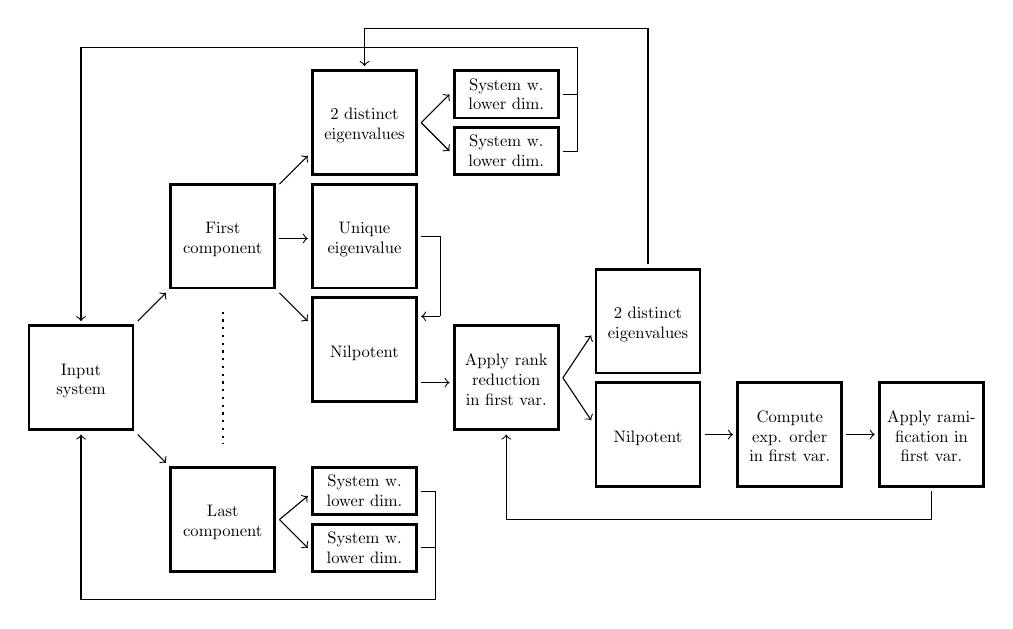
\begin{tikzpicture}[scale=0.6, every node/.style={scale=0.6}]
\draw [line width=1pt]
  (0,0) rectangle (2.2,2.2) node[label={[align=center]Input\\system}] at
  (1.1,0.4){ };

\path[->] (2.3,2.3) edge (2.9,2.9);
\path[->] (2.3,-0.1) edge (2.9,-0.7);

\draw [line width=1pt]
  (3,3) rectangle (5.2,5.2) node[label={[align=center]First\\component}] at
  (4.1,3.4){ };

\path[->] (5.3,5.2) edge (5.9,5.8);
\path[->] (5.3,4.05) edge (5.9,4.05);
\path[->] (5.3,2.9) edge (5.9,2.3);

\draw[thick,dotted] (4.1,2.5) -- (4.1,-0.3);

\draw [line width=1pt]
  (3,-3) rectangle (5.2,-0.8) node[label={[align=center]Last\\component}] at
  (4.1,-2.6){ };

\path[->] (5.3,-1.9) edge (5.9,-1.4);
\path[->] (5.3,-1.9) edge (5.9,-2.5);

\draw [line width=1pt] (6,-0.8) rectangle (8.2,-1.8)
node[label={[align=center]System w.\\lower dim.}] at (7.1,-1.9){ };

\draw [line width=1pt] (6,-2.0) rectangle (8.2,-3.0)
node[label={[align=center]System w.\\lower dim.}] at (7.1,-3.1){ };

\draw (8.3,-2.5) -- (8.6,-2.5) -- (8.6,-3.6) -- (1.1,-3.6);
\draw (8.3,-1.3) -- (8.6,-1.3) -- (8.6,-3.6);
\path[->] (1.1,-3.6) edge (1.1,-0.1);

\draw [line width=1pt] (6,5.4) rectangle (8.2,7.6)
node[label={[align=center] 2 distinct\\eigenvalues}] at (7.1,5.8){ };

\path[->] (8.3,6.5) edge (8.9,7.1);
\path[->] (8.3,6.5) edge (8.9,5.9);

\draw [line width=1pt]
  (6,3) rectangle (8.2,5.2) node[label={[align=center]Unique\\eigenvalue}] at
  (7.1,3.4){ };

\draw (8.3,4.1) -- (8.7,4.1) -- (8.7,2.4); 
\path[->] (8.7,2.4) edge (8.3,2.4);

\draw [line width=1pt]
  (6,0.6) rectangle (8.2,2.8) node[label={[align=center]Nilpotent}] at
  (7.1,1.2){ };

\path[->] (8.3,1.0) edge (8.9,1.0);

\draw [line width=1pt]
  (9,6.6) rectangle (11.2,7.6) node[label={[align=center]System w.\\lower dim.}] at
  (10.1,6.5){ };

  \draw [line width=1pt] (9,5.4) rectangle (11.2,6.4)
  node[label={[align=center]System w.\\lower dim.}] at (10.1,5.3){ };

\draw (11.3,7.1) -- (11.6,7.1) -- (11.6,8.1) -- (1.1,8.1); 
\draw (11.3,5.9) -- (11.6,5.9) -- (11.6,8.1); 
\path[->] (1.1,8.1) edge (1.1,2.3);

\draw [line width=1pt]
  (9,0) rectangle (11.2,2.2) node[label={[align=center]Apply rank\\reduction\\in
  first var.}] at
  (10.1,0.25){ };

\path[->] (11.3,1.1) edge (11.9,2.0);
\path[->] (11.3,1.1) edge (11.9,0.2);

\draw [line width=1pt] (12,1.2) rectangle (14.2,3.4)
node[label={[align=center] 2 distinct\\eigenvalues}] at (13.1,1.6){ };

\draw (13.1,3.5) -- (13.1,8.5) -- (7.1,8.5);
\path[->] (7.1,8.5) edge (7.1,7.7);

\draw [line width=1pt]
  (12,1.0) rectangle (14.2,-1.2) node[label={[align=center]Nilpotent}] at
  (13.1,-0.6){ };

\path[->] (14.3,-0.1) edge (14.9,-0.1);

\draw [line width=1pt]
  (15,1.0) rectangle (17.2,-1.2) node[label={[align=center]Compute\\ exp. order
    \\in first var.}] at
  (16.1,-0.95){ };

\path[->] (17.3,-0.1) edge (17.9,-0.1);

\draw [line width=1pt]
  (18,1.0) rectangle (20.2,-1.2) node[label={[align=center]Apply rami-\\
    fication in\\ first var.}] at
  (19.1,-0.95){ };

\draw (19.1,-1.3) -- (19.1,-1.9) -- (10.1,-1.9);
\path[->] (10.1,-1.9) edge (10.1,-0.1);
\end{tikzpicture}
\caption{Computing a fundamental matrix of formal solutions by working with one of
  the components, e.g. the first component. The other components would follow
  the chosen component in the uncoupling.}
\end{figure}
If the singularity is regular or one is interested in computing a full
fundamental matrix of formal solutions, as given by~\eqref{eq:sol}, then, besides
computing these invariants, further involved steps are required, as illustrated
in Example~\ref{ex:sim}. The recursive algorithm we propose generalizes that of
the univariate case given by the first author in~\cite{key24}. At each level of
recursion with input , we consider the leading matrix coefficients
 (we use both notation interchangeably) and distinguish
between three main cases:

\begin{enumerate}
\item There exists at least one index  such that
   has at least two distinct eigenvalues.
\item All of the leading matrix coefficients have exactly one eigenvalue and
  there exists at least one index  such that
   has a nonzero eigenvalue.
\item For all ,  is nilpotent.
\end{enumerate}
\vspace{0.3cm}

In order to identify the properties of the eigenvalues of , it
suffices to consider the constant matrix  due to the following
well-known proposition (see, e.g.,~\cite[Proposition 1, pp 8]{key4}
or~\cite[Proposition 2.2]{key9} for a proof within the context of eigenrings):
\begin{proposition}
\label{constev}
The eigenvalues of  , , belong to .
\end{proposition}
Then, based on the above classification, a linear or an exponential
transformation will be computed as described in the following subsections.

\subsection{Distinct Eigenvalues: Uncoupling the System Into Systems 
of Lower Dimensions}
\label{diagpfaff}
Whenever there exists an index  such that  has at
least two distinct eigenvalues, the system can be uncoupled into subsystems of
lower dimensions as shown in Theorem~\ref{blockpfaff}. For a constructive proof,
one may refer to~\cite[Section 5.2, pp 233]{key1}.
\begin{theorem}\label{blockpfaff}
  Suppose that for some , the leading matrix coefficient
   has at least two distinct eigenvalues. Then there exists a unique
  transformation  of the form
  
where , such that the transformation  yields
  the equivalent system
  
  and , 
  are of dimensions  and  respectively. 
\end{theorem}
The theorem can be restated by saying that if one of the components of the
system has a leading matrix coefficient with at least two distinct eigenvalues,
then it can be uncoupled. All of the other components are uncoupled
simultaneously. In the sequel, we aim to determine changes of the independent
variables  (ramifications), and construct transformations, which will allow
the reduction of any input system to a system for which the leading matrix
coefficient of at least one of its components has at least two distinct
eigenvalues. This allows us to either arrive at a system with lower Poincar\'e
rank or uncouple it into several subsystems of lower dimensions. The
recursion stops whenever we arrive at regular singular () or scalar
() subsystems. The former have been already investigated in~\cite[Chapter
3]{key73} and the resolution of the latter is straightforward.

We remark that, by Proposition~\ref{constev}, it suffices that there exists
 such that the constant matrix
 has at least two distinct
eigenvalues.

\subsection{Unique Eigenvalue: Shifting}
\label{shiftpfaff}
For any  such that  has a unique nonzero
eigenvalue , applying the so-called eigenvalue
shifting

yields a system  whose  component has a nilpotent leading
matrix coefficient:

The other components of the system are not modified by this transformation which
is clearly compatible with system .

Hence, due to the uncoupling and shifting, we can assume without
loss of generality that for all , the leading matrix
coefficients  are nilpotent.
\subsection{Nilpotency: Rank Reduction and Exponential Order}
\label{rampfaff}
In the univariate case, , the nilpotency of  suggests at least one
of the following two steps, as proposed by the first author in~\cite{key24}:
Rank reduction and computation of the exponential order . The
former reduces  to its minimal integer value. It is possible that 
drops to zero, i.e.\ we arrive at a regular singular system, or that the leading matrix
coefficient of the resulting system has at least two distinct eigenvalues, in
which case we can again uncouple the system. Otherwise,
 is to be computed, where~ and  are
coprime. Then, by setting  and applying rank reduction again, it
is proven that we arrive at a system whose leading matrix coefficient has two
distinct eigenvalues. Therefore, the system can be uncoupled (see
Figure~1).


The bivariate case, , is studied by the first and third authors of this
paper in~\cite{key101}. For rank reduction, the properties of principal ideal
domains were used. To determine the formal exponential order ,
associated univariate systems were defined. In this paper, we show that on the
one hand, this approach to determine the formal exponential order remains valid
in the multivariate setting, as we will see in the next section. On the other
hand, the generalization of the rank reduction algorithm to the multivariate
case is nontrivial and is discussed in Section~\ref{sec:rankred}. The
multivariate formal reduction algorithm is then summed up in
Section~\ref{mainpfaff}.

\section{Computing the Formal Invariants}
\label{sec:invariants}
In the univariate case, where the system is given by a single matrix ,
 can be computed from the characteristic polynomial of , i.e.\
, based on the analysis of a Newton polygon associated
with the system~\cite[Theorem 1]{key24}. In this section we show that one need
not search for a generalization of this algorithm to the multivariate case as
the formal invariants of , i.e.\ the exponential parts and , can
be obtained from an associated univariate system. We do not only give a method
to retrieve these invariants but we also reduce computations to computations
with univariate rather than multivariate formal series.
\begin{definition}
\label{defass}
Given a Pfaffian system , we call the following the \textit{associated ODS}
of :
  
  where
  
\end{definition}
\begin{theorem}
\label{exponentialpfaff}
For every , the -exponential part of a
Pfaffian system is equal to the exponential part of the 
component of its associated ODS.
 \end{theorem}
 To establish this result, we rely on a triangular form weaker than the
 Hukuhara-Turrittin's normal form given in Theorem~\ref{gerardexistence}. This
 weaker form suffices to give insight into the computation of~\eqref{eq:sol}.

 The following theorem is an reformulation of a theorem which was first given
 in~\cite[Proposition 3, pp 654]{key3} for the bivariate case, and then
 generalized in~\cite[Theorem 2.3]{key53} to the general multivariate case.
\begin{figure}
\label{fig2}
\centering
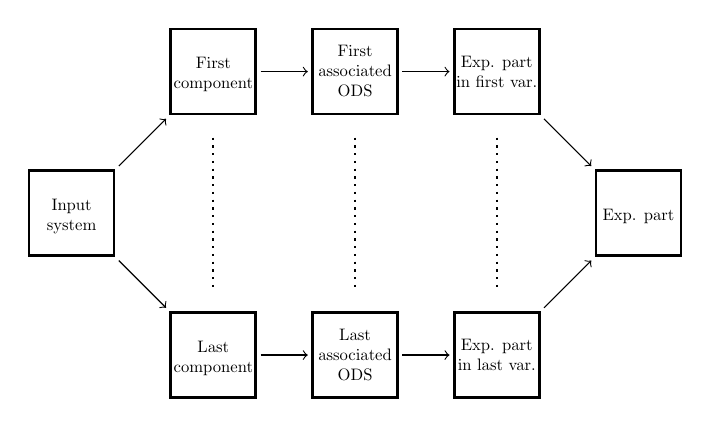
\begin{tikzpicture}[scale=0.6, every node/.style={scale=0.6}]
\draw [line width=1pt]
  (0,0) rectangle (1.8,1.8) node[label={[align=center]Input\\system}] at
  (0.9,0.2){ };

\path[->] (1.9,1.9) edge (2.9,2.9);
\path[->] (1.9,-0.1) edge (2.9,-1.1);

\draw [line width=1pt]
  (3,3) rectangle (4.8,4.8) node[label={[align=center]First\\component}] at
  (3.9,3.2){ };

\path[->] (4.9,3.9) edge (5.9,3.9);

\draw[thick,dotted] (3.9,2.5) -- (3.9,-0.7);

\draw [line width=1pt]
  (3,-3) rectangle (4.8,-1.2) node[label={[align=center]Last\\component}] at
  (3.9,-2.8){ };

\path[->] (4.9,-2.1) edge (5.9,-2.1);

\draw [line width=1pt] (6,3) rectangle (7.8,4.8)
node[label={[align=center]First\\associated\\ ODS}] at (6.9,3.1){ };

\path[->] (7.9,3.9) edge (8.9,3.9);

\draw[thick,dotted] (6.9,2.5) -- (6.9,-0.7);

\draw [line width=1pt] (6,-3) rectangle (7.8,-1.2)
node[label={[align=center]Last\\associated\\ ODS}] at (6.9,-2.9){ };

\path[->] (7.9,-2.1) edge (8.9,-2.1);

\draw [line width=1pt] (9,3) rectangle (10.8,4.8)
node[label={[align=center]Exp. part\\in first var.}] at (9.9,3.3){ };

\draw[thick,dotted] (9.9,2.5) -- (9.9,-0.7);

\draw [line width=1pt] (9,-3) rectangle (10.8,-1.2)
node[label={[align=center]Exp. part\\in last var.}] at (9.9,-2.7){ };

\path[->] (10.9,2.9) edge (11.9,1.9);
\path[->] (10.9,-1.1) edge (11.9,-0.1);

\draw [line width=1pt]
  (12,0) rectangle (13.8,1.8) node[label={[align=center]Exp. part}] at
  (12.9,0.4){ };
\end{tikzpicture}
\caption{Computing the exponential part from associated ODS's}
\end{figure}
\begin{theorem}
\label{gerardtransformation}
Consider the Pfaffian system . There exists a positive integer ,
and a transformation  (where  and
), such that the transformation  yields
the equivalent system:
7pt] x_i^{ \hat{p}_i+1} \pder{G}{x_i}= \hat{A}_{i}(x_2, \dots, x_n)\; G,
\quad 2 \leq i \leq n,
\end{cases}
2 & {\tilde{A}}_{1}(t_1, x_2, \dots, x_n) &\; =\;
  &\operatorname{Diag} (\hat{A}^{11}_{1}, \hat{A}^{22}_{1},
  \dots, \hat{A}^{jj}_{1}), \\
  &\hat{A}_{i}(x_2, \dots, x_n)& =\; & \operatorname{Diag}
  (\hat{A}^{11}_{i}, \hat{A}^{22}_{i}, \dots, \hat{A}^{jj}_{i}), \quad 2
  \leq i \leq n,
\hat{A}^{{\ell} {\ell} }_{1} = w^{{\ell} {\ell} }_{1} (t_1) I_{d_{\ell}
   } + t_1^{\alpha_1 \hat{p}_1}(\hat{N}^{{\ell} {\ell} }_{1}(x_2, \dots, x_n) +
   c^{{\ell} {\ell} }_{1} I_{d_{\ell}}),
t_1^{\alpha_1 \hat{p}_1 + 1} \pder{G}{t_1} = \tilde{A}_{1}(t_1, x_2, \dots, x_n)  \; G.

\label{relation}
t_1^{\alpha_1 {\hat{p}}_1 + 1}\pder{T}{t_1}= \alpha_1
A_{1}(x_1=t_1^{\alpha_1})\; T - T {\hat{A}}_{1}.
2 &\mathcal{A}_{1}(x_1=t_1^{\alpha_1}) &\;:=\; &A_{1} (x_1 =
  t_1^{\alpha_1}, x_2=0,\dots,x_n=0),\\ &\hat{\mathcal{A}}_{1} (t_1) &\; :=
  \;&\hat{A}_{1} (t_1, x_2=0, \dots, x_n=0),\\ &\mathcal{T} (t_1) &\; :=
  \;&T(t_1, x_2=0,\dots,x_n=0),

  t_1^{\alpha_1 \hat{p}_1 + 1} \pder{\mathcal{T}}{t_1} = \alpha_1
{\mathcal{A}}_{1}(x_1=t_1^{\alpha_1})\; \mathcal{T} - \mathcal{T}
{\hat{\mathcal{A}}}_{1}.

  p_{true}(A_i) - 1 < \omega(A_i)  \leq p_{true}(A_i).
  
  p_{true}(A_i) =p_{true}(\mathcal{A}_i).
p_{true}({\mathcal{A}}_{i}) -1 < \omega(A_i) = \omega({\mathcal{A}}_{i} ) \leq
    p_{true}({\mathcal{A}}_{i}).\qedhere
  m (A) = (m (A_1) , \dots, m (A_n)), & \text{where} &  m (A_{i}) =
\max\left(0, p_i + \frac{\operatorname{rank}(A_{i,0})}{d}\right),\\ 
\mu (A) = (\mu (A_1) , \dots, \mu (A_n)), & \text{where} &  \mu (A_{i})
= \operatorname{min}(\{ m (T(A_i)) \mid T \in GL_d({\rm R}_L) \}).

  x_i^{p_i +1 }\pder{F}{x_i} = A_i(x) F = (A_{i,0}({\bar{x}_i})+ A_{i,1}
({\bar{x}_i})x_i + A_{i,2}({\bar{x}_i}) x_i^2 + \dots ) F.
r:= \operatorname{rank} (A_{i,0}).
\label{eq:theta}
\theta_{i} (\lambda) := {x_i}^{r} \det(\lambda I + \frac{A_{i,0}}{x_i} + A_{i,1}
)|_{x_i=0}
 \label{ppp} \operatorname{m}(\tilde{A}_{i}) <
    \operatorname{m}(A_{i}) .S = \operatorname{Diag} (x_{i}^{\beta_1}, \dots , x_{i}^{\beta_d}),A_{1,0} = \left(\begin{matrix} 1 & 2 & 0 & 0 \\ 0 & 0 & 0 & 0 \\ -2 & 0 & 0 &
      0 \\ 0 & 1 & 0 & 0\end{matrix}\right)\quad\text{and}\quad A_{1,1} =
  \left(\begin{matrix} 4 & 9 & 2 & -5 \\ 8 & 9 & 0 & 0 \\ 8 & 6 & 2 & 4 \\ 5 & 6
      & 3 & 3\end{matrix}\right) . x_1^{p_1+1} \frac{\partial}{\partial x_1} F = \tilde{A_1} F \quad \text{where}
\quad \tilde{A_1} = S^{-1} A_1 S - x_1^p \operatorname{Diag}(1,1,0,0) .\tilde{A}_{1,0} = \left(\begin{matrix} 1 & 2 & 2 & -5 \\ 0 & 0 & 0 & 0 \\ 0
        & 0 & 0 & 0 \\ 0 & 0 & 0 & 0\end{matrix}\right),\ \ \tilde{A}_{1,1} =
    \left(\begin{matrix} 4 & 9 & * & * \\ 8 & 9 & * & * \\ -2 & 0 & 2 & 4 \\ 0 &
        1 & 3 & 3\end{matrix}\right).
\begin{cases} 
\tilde{A}_{i} = S^{-1} A_{i} S - x_{i}^{p_{i}}\operatorname{Diag}({\beta_1}, \dots ,
{\beta_d}), \\
\tilde{A}_{j}  = S^{-1} {A_{j}} S, \quad 1 \leq j \neq i \leq n , \end{cases}S^{-1} {A_{j}} S = \left(\begin{matrix} A_{j, 11} & A_{j,12}
      x_{i}^{\beta_2 - \beta_1} & \dots &  A_{j, 1d} x_{i}^{\beta_d - \beta_1} \5pt] \vdots & \vdots & \dots & \vdots
      \

The shearing in Example~\ref{ex:shearing} reduced the rank of the leading matrix
coefficient and was compatible with the system, i.e.\ it did not introduce
undesired denominators of , because of the column reduced form of
. The input system is not always given in such a
form for , and so we investigate in the following subsection how to
achieve it.

\subsection{Column Reduction}
\label{colpfaff}
To enable rank reduction, we alternate between the shearing transformation and
transformations which reduce some columns of a leading  matrix coefficient to
zero. For this we discuss in this section the following problem.

\medskip
\begin{quote}(P) \quad Given a square matrix
   (where
   denotes the th column) of rank  when considered as an element
  of , find a
  transformation  such that the last~ columns of
   are zero. \end{quote} 


\medskip
Before considering the algorithmic aspects,
we first discuss the existence of such a transformation. As the next example
shows, the desired transformation does not necessarily exist for any matrix .
\begin{example}
The matrix

is obviously of rank 1 over . There is, however, no
transformation~ such that  contains only one
non-zero column.
\end{example}
Consider the finitely generated -submodule
. We call it the column module of . In
order to construct a suitable transformation for bivariate Pfaffian systems (for
which the leading matrix coefficients are univariate) the authors
of~\cite{key101} use the fact that  and  are
principal ideal domains and hence that every finitely generated submodule of a
free module over this ring is free. We generalize this for the multivariate case
by showing in Corollary~\ref{cor:basis} that the freeness of the column module
 is a necessary and sufficient condition for the existence of a
transformation that meets our requirements. This is a direct consequence of
Nakayama's Lemma for local rings.

\begin{theorem} \cite[Theorem 2.3, pp 8]{key900}
  \label{theo:naka}
  Let  be a local ring,  its maximal ideal and let  be a
  finitely generated -module. Then  form a minimal
  set of generators for  if and only if their images
   under the canonical homomorphism
   form a basis of the vector space
   over the field .
\end{theorem}

The central consequence of Theorem~\ref{theo:naka} for us is that if  is
free, a module basis of  can be chosen among the columns of . We adapt the
theorem to our situation to show that we can bring  into a column-reduced
form if and only if its column module is free.

\begin{corollary}
  \label{cor:basis}
  Let  be of rank  over 
  and let  be the module generated by the columns of . If  is free,
  then there exists a subset  of the columns in  with  elements such
  that  is a module basis of . Furthermore,  is also a -vector
  space basis of the column space of .
\end{corollary}

\begin{proof}
  By Theorem~\ref{theo:naka} we can find a basis  of 
  among the columns of~. By definition, the  are linearly independent
  over , so they are also linearly independent over
   (otherwise, multiplying a linear relation in
   with a common denominator yields a relation in
  ). Since  is a basis of the column module, it also contains a
  generating set of the -vector space generated by
  the columns of .
\end{proof}

In theory, Corollary~\ref{cor:basis} would allow the computation of a unimodular
column reduction transformation as required in  simply via Gaussian
elimination. Assume we are given a matrix  and already know a subset
 of the columns of  which forms a basis of the column
module.  Let  be a column vector of  which is not in~. Then, since 
is a vector space basis, there exist  such that

By assumption,  is also a module basis, so there also exist
 with

The  are linearly independent, and therefore the cofactors of  with
respect to  are unique. It follows that  for all .


The main algorithmic difficulty stems from the fact that not all formal power
series admit a finite representation, and even if the initial system is given in
a finite form, the splitting transformation as in Theorem~\ref{blockpfaff} does
not preserve finiteness. In particular, we face two main problems when working
with truncated power series:
\begin{description}
\item [] Detecting the correct rank and the linear independent columns of
  
\item [] If we know the independent columns, a column reduction
  transformation computed after truncation is not uniquely determined.
\end{description}
These computational problems arise for general multivariate and for bivariate
systems, but were not addressed in previous algorithmic works on this
topic~\cite{key101,key5,key73}. Before we propose our resolution, we illustrate
both problems in the following example:

\begin{example}
\label{exm:trunc}
Consider the matrix 

Here, the first three columns  are linearly
independent and generate the column module. A linear combination of the fourth
column  is given by

When truncating at order 1, the system is given as 

The original rank cannot be determined from the truncated matrix. Furthermore,
even if we know that  are linearly independent, there are several
linear combinations of the fourth column after truncation:


The cofactors of the second linear combination are not the truncated cofactors
of the first. It can not be extended with higher order terms to a suitable linear
combination over the formal power series ring without truncation.
\end{example}

We can solve both  and  with the help of minors of the original
system. Let  be the rank of . Then there exists a nonzero 
submatrix  of  whose determinant is nonzero. Let  be the order of the
determinant. If we take the truncated system
, the same submatrix  in
 will have a non-zero determinant modulo  and we can
therefore identify in~ which columns in  are linearly
independent. This resolves  as long as the truncation order  is chosen
big enough.

Next assume that for instance the first  columns of  are linearly
independent, i.e.\ we can choose  such that its columns correspond to
. Let  be as above,  be a positive integer and let 
be a column vector that is linearly dependent on the columns of . Then there
exist  such that

By Cramer's rule, we know that the  are given by

where  is the matrix obtained by replacing the  column of  by
. Rewriting Equation~\eqref{cramer} gives

and this equation allows the computation of  by coefficient comparison. In
particular, we are guaranteed to obtain the correct  up to order  if
in~\eqref{cramer2} we replace  by , its truncation at order
, and  by , the truncation of  at order
. This resolves . 

This approach is based on the fact that there is a truncation order  such
that we can find a submatrix of maximal dimension with non-zero determinant. We
have to remark, however, that by the nature of formal power series, it is in
general not possible to tell a priori if a given truncation is high
enough.  Furthermore, we emphasize that it is in general not
  possible to draw a conclusion about the freeness of the column module from the
  integral relations among the truncated column vectors, since any linear
  combination of the form  can
  require a non-unit cofactor  for higher truncation orders. However, if no
  integral relations can be found with the above method, also the column module
  without truncation cannot be free. Both observations lead to the following
  practical approach. The full algorithm is carried out with a given truncation
  order. If the output is correct (compared to the invariant exponential part which can be obtained by Theorem~\ref{exponentialpfaff}), we are done. If not, we increase the
  truncation order until we get a correct output or arrive at a point where no
  integral relations can be found anymore.  This procedure necessarily
terminates, since there exists a suitable truncation order.  

One should note
that not every -vector space basis of the column space of  is also a
module basis. So, in the worst case,  submatrices have to be
tested to obtain a module basis.





\subsection{Converse of Theorem~\ref{moserpfaff}}

\label{proofpfaff}
We consider again a multivariate system  as in~\eqref{eq:sys}. We fix
 and investigate the rank reduction of its 
component given by

where the matrices  have their entries in  and the
algebraic rank of  is denoted by . We recall that we defined
 and .

The establishment of the converse of Theorem~\ref{moserpfaff} for the reduction in  follows
essentially the steps of that of the bivariate case which was given
in~\cite{key101}. The construction requires successive application of
transformations in  and shearing transformations in
. We remark that when applying a transformation
 on the  component,~\eqref{eq:gauge}
reduces to

Given~\eqref{first}, if the column module of  is free, then one can
compute a transformation  such that
  
  has rank , entries in  and with diagonal blocks of
  sizes  and  respectively. Let~ be the rank of
  .  If also the column module of  is free, then one
  can compute a transformation 
  such that
  
  has rank , entries in  and with diagonal blocks of
  sizes  and  respectively. We set
  .  Then the leading
  coefficient  of the equivalent system  has the
  following form:
5pt]
      \tilde{A}_{i,0}^{21} & O_{r-v}  & O \
with diagonal blocks of sizes ,   and
 respectively for some  and where 
5pt]
      \tilde{A}_{i,0}^{21} \end{matrix}\right) \quad \text{and} \quad
  \left(\begin{matrix}\tilde{A}_{i,0}^{11} & O \5pt] \tilde{A}_{i,0}^{31} & \tilde{A}_{i,0}^{32} \end{matrix}\right)
\label{glambdaformPfaffian} 
G_{A_{i}} (\lambda) := \left(\begin{matrix} A_{i,0}^{11} & O & A_{i,1}^{13}
    \5pt] A_{i,0}^{31} & A_{i,0}^{32} &
    A_{i,1}^{33}+ \lambda I_{d-r}\end{matrix}\right) . \det (G_{A_i}(\lambda)) & =& \det (N_0 + \lambda D_0) = \det
(N + \lambda D)|_{x_i=0} \\ & = & (\det(\frac{A}{x_i} + \lambda I_d) \det
(D))|_{x_i=0} \\ &=& (\det (\frac{A_{i,0}}{x_i} + A_{i,1} + \lambda I_d)
{x_i}^{r} )|_{x_i=0} = \theta_{i} (\lambda).   
\label{particularform3Pfaffian} 
G_{\tilde{A}_{i}} (\lambda) = \left(\begin{matrix} A_{i,0}^{11} & O & U_1& U_2
\5pt] V_1 & V_2 & W_1 + \lambda I_{d- r
-\varrho} & W_2 \ where ,
and
5pt] A_{i,0}^{21} &
      U_3 \5pt] A_{i,0}^{21} &
U_3 \end{matrix}\right), \5pt] A_{i,0}^{21} &
U_3 \end{matrix}\right) &<\; &r. 

\tilde{A}_{i,0} (\bar{x}_{i} ) = \left(\begin{matrix}
    O_{r}  & O \
Consequently, it can be easily verified that~\eqref{particularform3Pfaffian} is
given by
5pt] V_2 & W_1 +
    \lambda I_{d- r} \end{matrix}\right) , \quad \text{and} \quad \varrho = 0
. \begin{cases} S(x_i)=\operatorname{Diag}(x_i I_r , I_{d-r-\varrho}, x_i
   I_\varrho) \quad \text{if } \varrho \neq 0 \
 Furthermore, this shearing is compatible with system .
\end{proposition}
\begin{proof}
  Given system~\eqref{eq:sys}. For any  we partition
   according to~\eqref{particularform3Pfaffian}
5pt] A_{j}^{21} & A_{j}^{22} & A_{j}^{23} & A_{j}^{24}\5pt] A_{j}^{41} &
    A_{j}^{42} & A_{j}^{43} & A_{j}^{44}\end{matrix}\right), \quad 1 \leq j \leq
n, 2
  & \tilde{A}_{i} &= &\left(\begin{matrix}\phantom{x_i} A_{i}^{11}
      & \phantom{x_i} A_{i}^{12} & x_{i}^{-1} A_{i}^{13} & \phantom{x_i}
      A_{i}^{14} \5pt] x_{i} A_{i}^{31} &
      x_{i} A_{i}^{32}& \phantom{x_i^{-1}} A_{i}^{33}& x_{i} A_{i}^{34} \10pt] 
  & \tilde{A}_{j} &=& \left(\begin{matrix} \phantom{x_j} A_{j}^{11} & \phantom{x_j} A_{j}^{12} &
      x_{j}^{-1} A_{j}^{13} & \phantom{x_j} A_{j}^{14} \5pt] x_{j} A_{j}^{31}
      & x_{j} A_{j}^{32} & \phantom{x_j^{-1}}A_{j}^{33} & x_{j} A_{j}^{34} \ 
Hence, the leading matrix coefficient of the equivalent
-component is given by
5pt] A_{i,0}^{21} & O & U_3 & O \5pt]
    M_1 & O & M_3 & O \end{matrix}\right) 
 \label{eq:cond0}
 x_j^{p_j+1}\pder{A_{i,0}}{x_j}= A_{j}(x_i=0)\;A_{i,0} - A_{i,0} A_{j}(x_i=0) ,
\quad 1 \leq j \neq i \leq n .
 \label{form0} A_{i,0}({\bar{x}}_{i}) &=&\left(\begin{matrix}
A_{i,0}^{11} & O & O & O \5pt]
V_1 & V_2 & O_{(d-r-\varrho)(d-r-\varrho)} & O \10pt]
 \label{form1} A_{j}(x_i=0) &=& \left(\begin{matrix} A_{j}^{11}(x_i=0) &
A_{j}^{12}(x_i=0)& A_{j}^{13}(x_i=0)& A_{(j)}^{14}(x_i=0) \5pt] A_{j}^{31}(x_i=0) & A_{j}^{32}(x_i=0) &
A_{j}^{33}(x_i=0)& A_{j}^{34}(x_i=0)\ Inserting~\eqref{form0}
and~\eqref{form1} in~\eqref{eq:cond0}, one can obtain the desired results by
equating the entries of~\eqref{eq:cond0}. More explicitly, upon investigating
the entries in (Column 3), (Rows 1 and 2, Column 2), and (Row 4, Column 2), we
observe the following respectively:
\begin{itemize}
\item We have that 
5pt] A_{i,0}^{21} & O \5pt] M_1 & O \end{matrix}\right) \cdot \left(\begin{matrix}
A_{j}^{13}(x_i=0) \ The former matrix is of full rank  by construction thus  is a zero matrix.
\item We also get
 The former is of full rank  by
construction thus  is a zero matrix.
\item Finally, . Since  is null and  is of full
column rank  by construction then  is a zero matrix as
well.
\end{itemize} This completes the proof.\end{proof}

We can thus establish the following theorem:

\begin{theorem}
\label{moserpfaff2}
Consider a Pfaffian system~ and suppose that  for some index . If  given by~\eqref{eq:theta} vanishes for some index , then under the conditions required to attain~\eqref{gaussformPfaffian} and Proposition~\ref{gauss3Pfaffian}, we can
construct a compatible transformation  which reduces
 (and consequently ). In this case,  can be chosen to be a
product of transformations in  and polynomial
transformations of the form
 where
 are non-negative integers.
\end{theorem}

\begin{proof}
Under the required conditions, we can assume that  has the
  form~\eqref{gaussformPfaffian}. Let  be given by~\eqref{glambdaformPfaffian}. Then
   vanishes identically in  if and only
  if  does. Then the system  where
   are as in Propositions~\ref{gauss3Pfaffian} and~\ref{shearingPfaffian}
  respectively, has the desired property.
\end{proof}
For a given index , the algebraic rank of the leading matrix coefficient can be decreased as long as  vanishes
identically in . In case the leading matrix coefficient eventually
reduces to a zero matrix, the Poincar\'e rank drops at least by one. This
process can be repeated until the Moser rank of system  equals to its Moser
invariant. Due to the compatibility of  in Theorem~\ref{moserpfaff}, rank
reduction can be applied to any of the components of  without altering the
Moser rank of the others. Hence, by Corollary~\ref{prank}, the true Poincar\'e
rank of system~ can be attained by a successive application of the rank
reduction to each of its components.

Finally, we remark that the conditions of Theorem~\ref{moserpfaff2} are always satisfied in the bivariate case  of arbitrary dimension.

\subsection{Examples}
\begin{example}
Consider the completely integrable Pfaffian system with normal crossings given by 
  
A fundamental matrix of formal solutions is given by:
 
    
If we only seek to compute the exponential parts  in~\eqref{exm3:sol}, then from the associated ODS, we compute:


Furthermore, if we wish to compute a fundamental matrix of formal solutions,
then following the steps of our formal reduction algorithm, we look at the
leading coefficients of each of the three components of the given system. If one
of these coefficients has two distinct eigenvalues, the we can apply the
splitting lemma (Theorem~\ref{blockpfaff}). Indeed, since  has this property, we can
compute such a transformation  up to any order. In particular, up to
order , we compute:

which yields the following diagonalized system (up to order ):


with .
Hence, the system can be uncoupled into two subsystems of linear scalar
equations and integrated to construct , and consequently,~.
\end{example}

An example of the reduction process for a system in two variables was given in
Example~\ref{ex:sim}. However, examples of dimensions two and three do not cover
the richness of the techniques presented. So, to illustrate the full process, we
treat an example of dimension six. Due to the size of the system and the number
of necessary computation steps, we are not able to include it directly in this
paper. It is available in several formats at \vspace{0.1cm}
\begin{center}
\url{http://www.mjaroschek.com/pfaffian/}
\end{center}
\section{Formal Reduction Algorithm}
\label{mainpfaff}
\subsection{The Algorithm In Pseudo Code}
We now give the full algorithm in pseudo-code and we refer to more
detailed descriptions within the article whenever necessary.

\begin{remark}
  Throughout the article, we adopted the field of complex numbers  as
  the base field for the simplicity of the presentation. However, any computable
  commutative field  with  can
  be considered instead. In this case, the restrictions on the extensions of the
  base field discussed in~\cite{key24} apply
  as well and are taken into consideration within our \textsc{Maple}
  implementation.
\end{remark}

Given system , we discuss the eigenvalues of the leading matrix coefficients 
, , of its  components. If for all of these
components uncoupling is unattainable, then we fix  and
proceed to compute the exponential order  from the associated ODS.
Suppose that  with  coprime positive
integers. One can then set  (re-adjustment of the independent
variable), and perform again rank reduction to get an equivalent system whose
 component has Poincar\'e rank equal to  and leading matrix
coefficient with at least  distinct eigenvalues. Consequently,
block-diagonalization can be re-applied to uncouple the -component.  By
Section~\ref{diagpfaff}, this uncoupling results in an uncoupling for the
whole system. As mentioned before, this procedure can be repeated until we
attain either a scalar system, i.e.\ a system whose  components are scalar
equations, or a system whose Poincar\'e rank is given by . The
former is trivial and effective algorithms are given for the latter
in~\cite[Chapter 3]{key73}. \vspace{1cm}

\bgroup
\def\arraystretch{1.0}
\begin{center}
  \begin{tabular}{p{11cm}l}
    \hline\-2.5ex]
    \begin{tabular}{lp{9cm}}
      \textbf{Input:} &  of~\eqref{eq:sys}.\\
      \textbf{Output:} & A fundamental matrix of formal solutions~\eqref{eq:sol}.\\
    \end{tabular} & \\
    \hline\-2.5ex]
    \textbf{Algorithm 2: rankReduce(}\textbf{)}\\
    \hline\-2.5ex]
    \begin{tabular}{ll}
\quad  \\
\quad  \textbf{FOR} every  from  to  \textbf{DO}\\
\quad \quad  ;  Poincar\'e rank of  \\
\quad \quad   yields the
      form~\eqref{gaussformPfaffian} \\
\quad \quad \textbf{IF}  cannot be determined \\
 \quad \quad\quad \textbf{RETURN
     ERROR} ``Column module not free.'' \textbf{END IF}\\
 \quad \quad   ;  \\
 \quad \quad  \textbf{WHILE}  and  \textbf{DO} \\
 \quad \quad \quad 
      Proposition~\ref{gauss3Pfaffian} \\
 \quad \quad \quad \textbf{IF}  cannot be determined \\
 \quad \quad \quad\quad \textbf{RETURN
     ERROR} ``Row module not free.'' \textbf{END IF}\\
 \quad \quad \quad  Proposition~\ref{shearingPfaffian} \\
 \quad \quad \quad ;  \\
 \quad \quad \quad  \\
 \quad \quad \quad  Poincar\'e rank of  \\
 \quad \quad \quad   yields the form~\eqref{gaussformPfaffian}  \\
 \quad \quad \quad ;  \\
 \quad \quad \textbf{END WHILE} \\
\quad \quad \textbf{FOR} every  from  to  \textbf{DO}\\
\quad \quad \quad  \\
\quad \quad \textbf{END FOR}\\
\quad \quad  \\
\quad \textbf{END FOR}\\
\quad \textbf{RETURN} ().
    \end{tabular} & \\
    \hline
  \end{tabular}
\end{center}
\egroup

\subsection{An Alternative Rank Reduction Algorithm}
\label{sec:alt}
In the case of univariate systems, Levelt's investigations of the existence of
stationary sequences of free lattices lead to an algorithm which reduces the
Poincar\'e rank to its minimal integer value~\cite{key57}. This algorithm was
then generalized to the bivariate case by the first author of this paper et
al. in~\cite{key5}. The theoretical basis of this algorithm differs
substantially from the algorithm given herein based on Moser's criterion. The
final result of both approaches however, i.e.\ the algorithm itself, is based on
applying column reductions and shearing transformations in both algorithms,
though in a different manner. In fact, the algorithms coincide for the
particular case of . The limitation in~\cite{key5} within the
generalization to the multivariate case is in guaranteeing the freeness
conditions for the leading matrix coefficient  as stated in
Section~\ref{proofpfaff}. The additional condition of the freeness of the row
module as in Proposition~\ref{gauss3Pfaffian} is not required. Since the linear algebra
problem is resolved in Section~\ref{colpfaff}, this results in Algorithm~.

Although both algorithms have an identical cost~\cite[pp 108]{key73},
experimental results for the univariate case and certain bivariate systems
(singularly-perturbed linear differential systems) suggest that the
lattice-based algorithm complicates dramatically the coefficients of the system
under reduction, even if Moser's criterion is adjoined to avoid some unnecessary
computations~\cite[Section 4.3]{key102}. Hence, Algorithm~ can be used as
long as the required freeness conditions hold. Nevertheless, if the freeness of
the row module of  is not satisfied, then Algorithm~ can
be used as long as the column modules of  and  is free.  There remains
however, the question on the equivalence of these conditions.

\bigskip
\bgroup
\def\arraystretch{1.0}
\begin{center}
  \begin{tabular}{p{11cm}l}
    \hline\-2.5ex]
    \begin{tabular}{lp{9cm}}
    \textbf{Input:} &  of~\eqref{eq:sys}.\\
    \textbf{Output:} &  and an irreducible equivalent system
                       \{\} whose Poincar\'e rank is its true
                       Poincar\'e rank and the rank of its leading coefficient
                       matrices is minimal ()\\
    \end{tabular} & \\
    \hline\-2.5ex]
    \begin{tabular}{ll}
\quad  \\
\quad  \textbf{FOR} every  from  to  \textbf{DO}\\
\quad \quad  ;  Poincar\'e rank of  \\
\quad \quad \textbf{WHILE}  and  \textbf{DO} \\
\quad \quad \quad   yields the form
      \eqref{gaussformPfaffian} \\
\quad \quad \quad \textbf{IF}  cannot be determined \\
 \quad\quad \quad\quad \textbf{RETURN
     ERROR} ``Column module not free.'' \textbf{END IF}\\
 \quad \quad  \quad    \\
 \quad \quad  \quad    Proposition~\ref{shearingPfaffian} with  (i.e.\ )\\
 \quad \quad  \quad   \\
 \quad \quad \quad   \\
 \quad \quad \quad   Poincar\'e rank of  \\
 \quad \quad \quad   \textbf{IF}   \textbf{THEN} \\
 \quad \quad \quad   \quad  \\
 \quad \quad \quad   \textbf{ELSE}\\
 \quad \quad \quad   \quad  \\
 \quad \quad \quad  \textbf{END IF}\\
 \quad \quad \quad   \\
\quad \quad \quad  \\
\quad \quad \textbf{END WHILE} \\
\quad \quad \textbf{FOR} every  from  to  \textbf{DO}\\
\quad \quad \quad  \\
\quad \quad \textbf{END FOR}\\
\quad \quad  \\
\quad \textbf{END FOR}\\
\quad \textbf{RETURN} ().
    \end{tabular} & \\
    \hline
  \end{tabular}
\end{center}
\egroup

\goodbreak
\section{Conclusion}
\label{conpfaff}
In this article, we studied completely integrable Pfaffian systems with normal
crossings in several variables. We showed that one can associate a set of
univariate linear singular differential systems from which the formal invariants
of the former can be retrieved. This reduces computations to computations over a
univariate field via \textsc{Isolde} or \textsc{Lindalg}, and limits the numbers
of coefficients necessary for the computations. We then complemented our work
with a rank reduction algorithm based on generalizing Moser's criterion and the
algorithm given by Barkatou in~\cite{key41}. The former is applicable to any
bivariate system. However, for multivariate systems, it demands that several explicitly
described conditions are met.

One field of investigation is the possibility of weakening the conditions required in the multivariate setting for the rank reduction. Another one is the adaptation of the techniques developed herein for rank reduction to generalize the notion of \textit{simple} systems (see~\cite{key40} for
). This notion, in the univariate case, gives another approach to construct a basis of the space of regular
solutions~\cite{key25}, and the obstacles encountered are similar to those in rank reduction. An additional field is to study closed form solutions~\cite{key3811}
in the light of associated ODS introduced in Section~\ref{sec:invariants}. 

In future work we aim
to thoroughly study the theoretical complexity of the proposed algorithm as well
as give detailed information of the effects on the truncation of the input
system during the computation. This work is not straightforward and even in the
case of regular systems, it is
not studied in the existing work (i.e. ~\cite[Chapter 3]{key73} and references therein). 

Systems arising from applications do not necessarily or directly fall into the
class of completely integrable Pfaffian systems with normal
crossings. Investigations in more general classes can be found
in~\cite{key32,key3062,key4092} and references therein. 

An additional field of investigation is the formal reduction in the difference
case using the approaches proposed herein. Praagman established
in~\cite{key3239} a formal decomposition of  commuting partial linear
difference operators. This study was intended as an analog to that established
by Levelt, van den Essen, G\'erard, Charri\`ere, Deligne, and
others~\cite{key3,key53,key20,key21}. 

\section*{Acknowledgments}
\label{Ack}
We are grateful to the anonymous referees whose comments and suggestions
improved the readability of this paper. The second author would also like to
thank the Technische Universit\"at Wien, where he is employed by the time of
submission and supported by the ERC Starting Grant 2014 SYMCAR 639270. He
furthermore would like to thank Matteo Gallet for valuable discussions. The
third author would like to thank the University of Limoges since a part of this
work was done during the period of her doctoral studies at DMI.


\bibliographystyle{plain}
\begin{thebibliography}{00}
\bibitem{key101} H. Abbas, M. Barkatou, and S.S. Maddah. Formal Solutions of a
  Class of Pfaffian Systems in Two Variables. In \textit{Proceedings of the
    International Symp. on Symb. and Algeb. Comp.}, ACM Press, pp 312-319, 2014.
\bibitem{key102} H. Abbas, M. A. Barkatou, and S.S. Maddah. On the Reduction of Singularly-Perturbed Linear Differential Systems. In \textit{Proceedings of the 39th International Symposium on Symbolic and Algebraic Computation}, ACM Press, pp 320-327, 2014.
\bibitem{key3908} A. Aparicio Monforte and M. Kauers, Formal Laurent Series in
  Several Variables, \textit{Expositiones Mathematicae}, 31(4):350--367,
  December 2013,
  \bibitem{key3701} D. G. Babbitt and V. S. Varadarajan. Formal Reduction of Meromorphic Differential Equations: A Group Theoretic View. In \textit{Pacific Journal of Mathematica}, 109 (1), pp 1- 80, 1983.
\bibitem{key6} W. Balser. \textit{Formal Power Series and Linear Systems of
    Meromorphic Ordinary Differential Equations}. Springer, 2000.
\bibitem{key24} M. Barkatou. An algorithm to compute the exponential part of a
  formal fundamental matrix solution of a linear differential
  system. \textit{Journal of App. Alg. in Eng. Comm. and Comp.}, 8(1):1-23,
  1997.
\bibitem{key41} M. Barkatou. A Rational Version of Moser's Algorithm. In
  \textit{Proceedings of the International Symposium on Symbolic and Algebraic
    Computation}, pages 297-302. ACM Press, July 1995.
    \bibitem{key9} M. Barkatou. Factoring systems of linear functional equations using eigenrings. In I. S. Kotsireas and E. V. Zima, editors, \textit{Latest Advances in Symbolic Algorithms}, pp 22--42. World Scientific, 2007.
     \bibitem{B10}  M. Barkatou. Symbolic methods for solving systems of linear ordinary differential equations. Tutorial at the
  \textit{International Symposium on Symbolic and Algebraic
    Computation}, pages 7-8. ACM Press, July 2010.
    \bibitem{key3811} M. A. Barkatou,  T. Cluzeau, C. El Bacha, and J. A. Weil. Computing closed form solutions of integrable connections. In \textit{Proceedings of the 37th International Symposium on Symbolic and Algebraic Computation}, pp 43-50, ACM press, 2012.
\bibitem{key40} M. Barkatou and C. El Bacha. On k-simple forms of first-order
  linear differential systems and their computation. \textit{Journal of
    Symb. Comp.},54:36-58, 2013.
\bibitem{key25} M. Barkatou and E. Pfluegel. An algorithm computing the regular
  formal solutions of a system of linear differential equations. \textit{Journal
    of Symbolic Computation}, 28(4), 569-587, 1999.
\bibitem{key26} M. Barkatou and E. Pfluegel. Computing super-irreducible forms of systems of linear differential equations via moser-reduction: a new approach. In \textit{Proceedings of the 2007 international symposium on Symbolic and algebraic computation}, pp. 1-8. ACM, 2007.
\bibitem{key27} M. Barkatou and E. Pfluegel. ISOLDE, Integration of Systems of
  Ordinary Linear Differential Equations. Available at:
  http://isolde.sourceforge.net/
\bibitem{key5} M. Barkatou and N. LeRoux. Rank Reduction of a class of Pfaffian
  Systems in Two Variables. In \textit{Proceedings of the International Symposium
    on Symbolic and Algebraic Computation}, pages 204-211. ACM Press, 2006.
\bibitem{key31} R. Broucke. On Pfaff's equations of motion in dynamics;
  Applications to Satellite Theory. \textit{Journal of Celestial Mechanics},
  18(3): 207-222, 1978.
\bibitem{key3} H. Charri\`{e}re. Triangulation Formelle de certains Syst\`{e}mes
  de Pfaff Compl\`{e}tement Int\'{e}grables et Application \`{a} l'etude
   des Syst\`{e}mes non Lin\'{e}aires. \textit{Annali della Scuola
    Normale Superiore di Pisa-Classe di Scienze}, 7(4): 625 - 714, 1980.
\bibitem{key53} H. Charri\`ere and R. G\'erard. Formal Reduction of Integrable
  Linear Connexion having a certain kind of Irregular
  Singularities. \textit{Analysis}, 1:85-115, 1981.
\bibitem{key20} P. Deligne. Equations Diff\'{e}rentielles \`{a} Points
  Singuliers R\'{e}guliers. \textit{Lecture Notes In Mathematics}, Volume 163,
  Springer-Verlag,1970.
    \bibitem{key74} D. Delphenich. The role of integrability in a large class of physical systems. \textit{arXiv preprint avilable at:} arXiv:1210.4976 (2012).
\bibitem{key21} A. van den Essen. Regular Singularities along Normal
  Crossings. In Gerard Ramis, editor, \textit{Syst\`{e}mes de Pfaff et Equations
    Diff\'{e}rentielles dans le Champ Complexe}, volume 712 of \textit{Lecture Notes
    in Mathematics}, pages 88-130. Springer-Verlag, 1979.
\bibitem{key4} A. van den Essen and A.H.M. Levelt. Irregular Singularities in
  Several Variables. \textit{Memoirs of AMS}, 40(270), 1982.
\bibitem{key1} R. G\'{e}rard and Y. Sibuya. Etude de certains syst\`{e}mes de
  Pfaff avec singularit\'{e}s.  In Gerard Ramis, editor, \textit{Systemes de Pfaff
    et Equations Diff\'{e}rentielles dans le Champ Complexe}, volume 712 of
  \textit{Lecture Notes in Mathematics}, pages 131-288. Springer-Verlag, 1979.
\bibitem{key3062} H. Hashiguchi, Y. Numata, N. Takayama, and A. Takemura. The
  Holonomic Gradient Method for the Distribution Function of the Largest Root of a
  Wishart Matrix. \textit{Journal of Multivariate Analysis}, volume 117, pp 296 -
  312, 2013.
\bibitem{key73} N. LeRoux. Solutions formelles d'\'equations aux d\'eriv\'ees
  partielles. Ph.D. Thesis. University of Limoges. 2006.
\bibitem{key57} A.H.M. Levelt. Stabilizing Differential Operators: a method for
  Computing Invariants at Irregular Singularities. \textit{Differential Equations
    and Computer Algebra, M. Singer (ed.)}, pages 181-228, 1991.
    \bibitem{key3702} D. A. Lutz and R. Schaefke. On the Identification and Stability of Formal Invariants for Singular Differential Equations. In \textit{Linear Algebra and its Applications}, 72, pp 1- 46, 1985. 
\bibitem{key427} S. S. Maddah. Mathemagix Lindalg Package for Symbolic
  Resolution of Linear Systems of Differential Equations. Available at:
  
\bibitem{key900} H. Matsumura. \textit{Commutative Ring Theory}. Cambridge
  Studies in Advanced Mathematics, Cambridge University Press, ISBN 9780521367646,
  1989. Available at: 
\bibitem{key19} J. Moser. The Order of a Singularity in Fuchs' Theory.
  \textit{Mathematische Zeitschrift}, 72:379- 398, 1960.
\bibitem{key32} D. Novikov, S. Yakovenko. Lectures on meromorphic flat
  connections. \textit{Normal forms, bifurcations and finiteness problems in
    diff-l eqn.}, pages 387-430, 2004.
    \bibitem{key3239} C. Praagman. Formal Decomposition of  Commuting Partial Linear Difference Operators. \textit{Rijksuniversiteit Groningen, Mathematisch Instituut}, 1983.
    \bibitem{key4092} K. Takano. Local Equivalence of Linear Pfaffian Systems with Simple Poles. \textit{Funkcialaj Ekvacioj}, 24, 373-382, 1981.
\bibitem{key7} W. Wasow. \textit{Asymptotic Expansions for Ordinary Differential
    Equations}. Dover Publications, 2002.


\end{thebibliography}
\end{document}
